\documentclass{iacrtrans}
\usepackage[utf8]{inputenc}

\author{Cube Labs}
\institute{contact@cube.network}
\title[\texttt{Cube}: A High-Performance Modular Blockchain Supporting Multi-chain Architecture
]{\publname}

\usepackage{fancyhdr}
\pagestyle{plain}
\fancyfoot[C]{\thepage} % 页码

\begin{document}

\maketitle

\keywords[]{Cube\and Blockchain\and Collaborative-rollup\and Chaos consensus\and Data availability sharding\and Time crossing}

\begin{abstract}
	In this paper, we propose a high-performance modular blockchain that supports a multi-chain structure. With the popularity of crypto increasing every day, scalability has become the biggest challenge for permissionless blockchains. At present, the common way to solve the scaling problem is to optimize its monolithic structure, whereas, \texttt{Cube} proposes the layered architecture by vertically segmenting settlement, execution, and data availability into three different layers and optimizing each one of them according to their specifics. \texttt{Cube} also proposes a collaborative ZK-Rollup and “Chaos Consensus” protocol. In addition, \texttt{Cube} has designed a “Time Crossing” cross-chain protocol fully compatible with the Cosmos ecosystem. With the proposed structure \texttt{Cube} can reach hundreds of thousands of TPS and eliminate the need for external data availability for Rollup and NFT, thus providing an efficient and reliable full-stack solution for the development of Web 3.0.
\end{abstract}

%\tableofcontents{}

\section{Introduction}\label{Introduction}
Since the introduction of Bitcoin [4], blockchain technology and the idea of decentralization have gradually gained popularity. Ethereum [5] and its smart contracts gave almost unlimited application for distributed ledger technology. However, the main concerns of early blockchain technology were security and decentralization while transaction processing capacity was not considered enough. The transaction processing capacity of about a dozen TPS has greatly limited the further development of blockchain applications, considering the present scenario, with the explosive growth of decentralized applications such as DeFi, GameFi, and NFT, the number of transactions submitted to the permissionless blockchains have increased exponentially. At peak traffic, the gas price of the Ethereum network can reach thousands of Gwei and a single transaction can cost a user a hundred of dollars in transaction fees. The transaction processing capacity of permissionless blockchains is becoming a bottleneck for the continued growth of the decentralized economy.

In order to solve the problem of scaling in permissionless blockchain, numerous technological advancements and solutions have been proposed and applied [6,7,8,9,10,11,12,13], some of which are based on multi-chain architecture and some on state sharding. Those techniques alleviate the pressure of scaling to some extent. Still, this horizontal splitting causes fragmentation of the whole system and sacrifices some security and decentralization features and still does not solve the scaling problem. Meanwhile, there are also Layer 2-based scaling solutions, such as Rollup [15], Plasma [14], State Channels [16], etc, which made progress in scalability but were not systematic and thorough.

From a functional point of view, the whole blockchain system consists of three parts:
\begin{itemize}
	\item[$\bullet$] Execution of transactions;
	\item[$\bullet$] Verification and consensus on the results of transaction execution;
	\item[$\bullet$] Storage of the original data of the transaction.
\end{itemize}

The specifics of each part are different. Putting those together to optimize will inevitably lead them to conflict with each other. Optimization can be achieved only if the entire system is vertically split in the above functions according to their specifics.

Here we propose \texttt{Cube}, a next-generation modular blockchain with a multi-chain architecture, that is secure, fast and scalable. We believe that \texttt{Cube} makes a more systematic and thorough vertical splitting of blockchain which is necessary to solve the scaling problem mentioned above fundamentally. \texttt{Cube} is designed with the execution layer for transaction execution by using the ZK Rollup-based Validium solution and a self-developed Collaborative Rollup solution as the system's execution engine. In terms of consensus, \texttt{Cube} is designed with a settlement layer that is fully compatible with EVM and Ethereum protocols and introduces a high-performance consensus protocol that supports large-scale node participation. In terms of raw data storage for transactions, \texttt{Cube} is designed with a data availability layer that implements block data sharding and sampling validation schemes to provide efficient and reliable storage services. For Rollup and NFT applications, there is no need to rely on external storage solutions any longer since the processing logic and data are fully managed. In addition, \texttt{Cube} does not forget about multi-chain support and has developed a decentralized cross-chain communication protocol named “Time Crossing”, which supports cross-chain DeFi contract calls and is compatible with Cosmos IBC protocol.

\texttt{Cube} is a public blockchain that is designed to collaborate and promote the development of the industry, taking into account the current needs of decentralized applications and the future innovation and development. It takes high-performance underlying permissionless blockchain as a new starting point, realizes the ultimate performance optimization of single-chains in phases, supports and promotes the development of Web 3.0 in modular layers, solves storage pain points, forming a permissionless blockchain with complete underlying capabilities that everyone can participate in. Furthermore, it actively leads and participates in the development and construction of decentralized cross-chain protocols to form a multi-chain network and integrate itself into the new world of interconnected chains to become an indispensable part of the metaverse infrastructure. 

Compared with other permissionless blockchains, \texttt{Cube} is committed to making innovations and contributions in blockchain scaling and cross-chain, and also addressing the full-stack requirements of Web 3.0, with the following five core technical features.
\begin{itemize}
	\item[$\bullet$] Modular layered architecture, built-in Rollup, and extreme scaling, supporting hundreds of thousands of TPS;
	\item[$\bullet$] Pipelined optimized BFT consensus, combining high throughput, decentralization, secure and fast transaction confirmation;
	\item[$\bullet$] Full compatibility with Ethereum protocols and EVM, supporting a seamless migration of applications within the ecosystem
	\item[$\bullet$] Built-in data availability solutions to address Web 3.0 full-stack requirements;
	\item[$\bullet$] Support DeFi cross-chain calls, multi-chain network structure and compatible with Cosmos IBC, interconnecting all chains.
\end{itemize}

\section{Overall Architecture}
In the field of traditional permissionless blockchain scaling, there has been the Blockchain Trilemma of decentralization, security and scalability that no current blockchain system can simultaneously achieve. 

\texttt{Cube} believes that the solution lies in the fact that the traditional blockchain has monolithic architecture, which means components are interconnected and interdependent. You couldn't just take a piece of it and plug it into something else. 

To solve this problem, \texttt{Cube} adopts a modular architecture which is divided into three layers: Execution Layer, Settlement Layer and Data Availability Layer.

\begin{itemize}
	\item[$\bullet$] Execution Layer: responsible for the execution of almost all contract-based transactions and supports decentralized applications. It is the combination of ZK Rollup and Collaborative Rollup, where the execution results are submitted to the settlement layer and the settlement layer establishes undeniable security as well as objective finality. 
	\item[$\bullet$] Settlement layer: responsible for verifying and settling the execution results of the execution layer and is also the asset layer, responsible for the management and settlement of the assets on the chain.
	\item[$\bullet$] Data availability layer: focusing on data storage, it will store permanently high-value data based on data sharding, and with data availability sampling technologies it can support reliable verification for light clients.
\end{itemize}

In addition, relying on our Time Crossing cross-chain protocol, \texttt{Cube} can also implement multi-chain topology to meet the demand for application chains. Meanwhile, “Time Crossing” is also compatible with Cosmos IBC to achieve cross-chain support for blockchains in the Cosmos ecosystem and Cosmos Hub. The overall system architecture is illustrated in Figure \ref{fig:1}.

\begin{figure}[h]
	\centering
	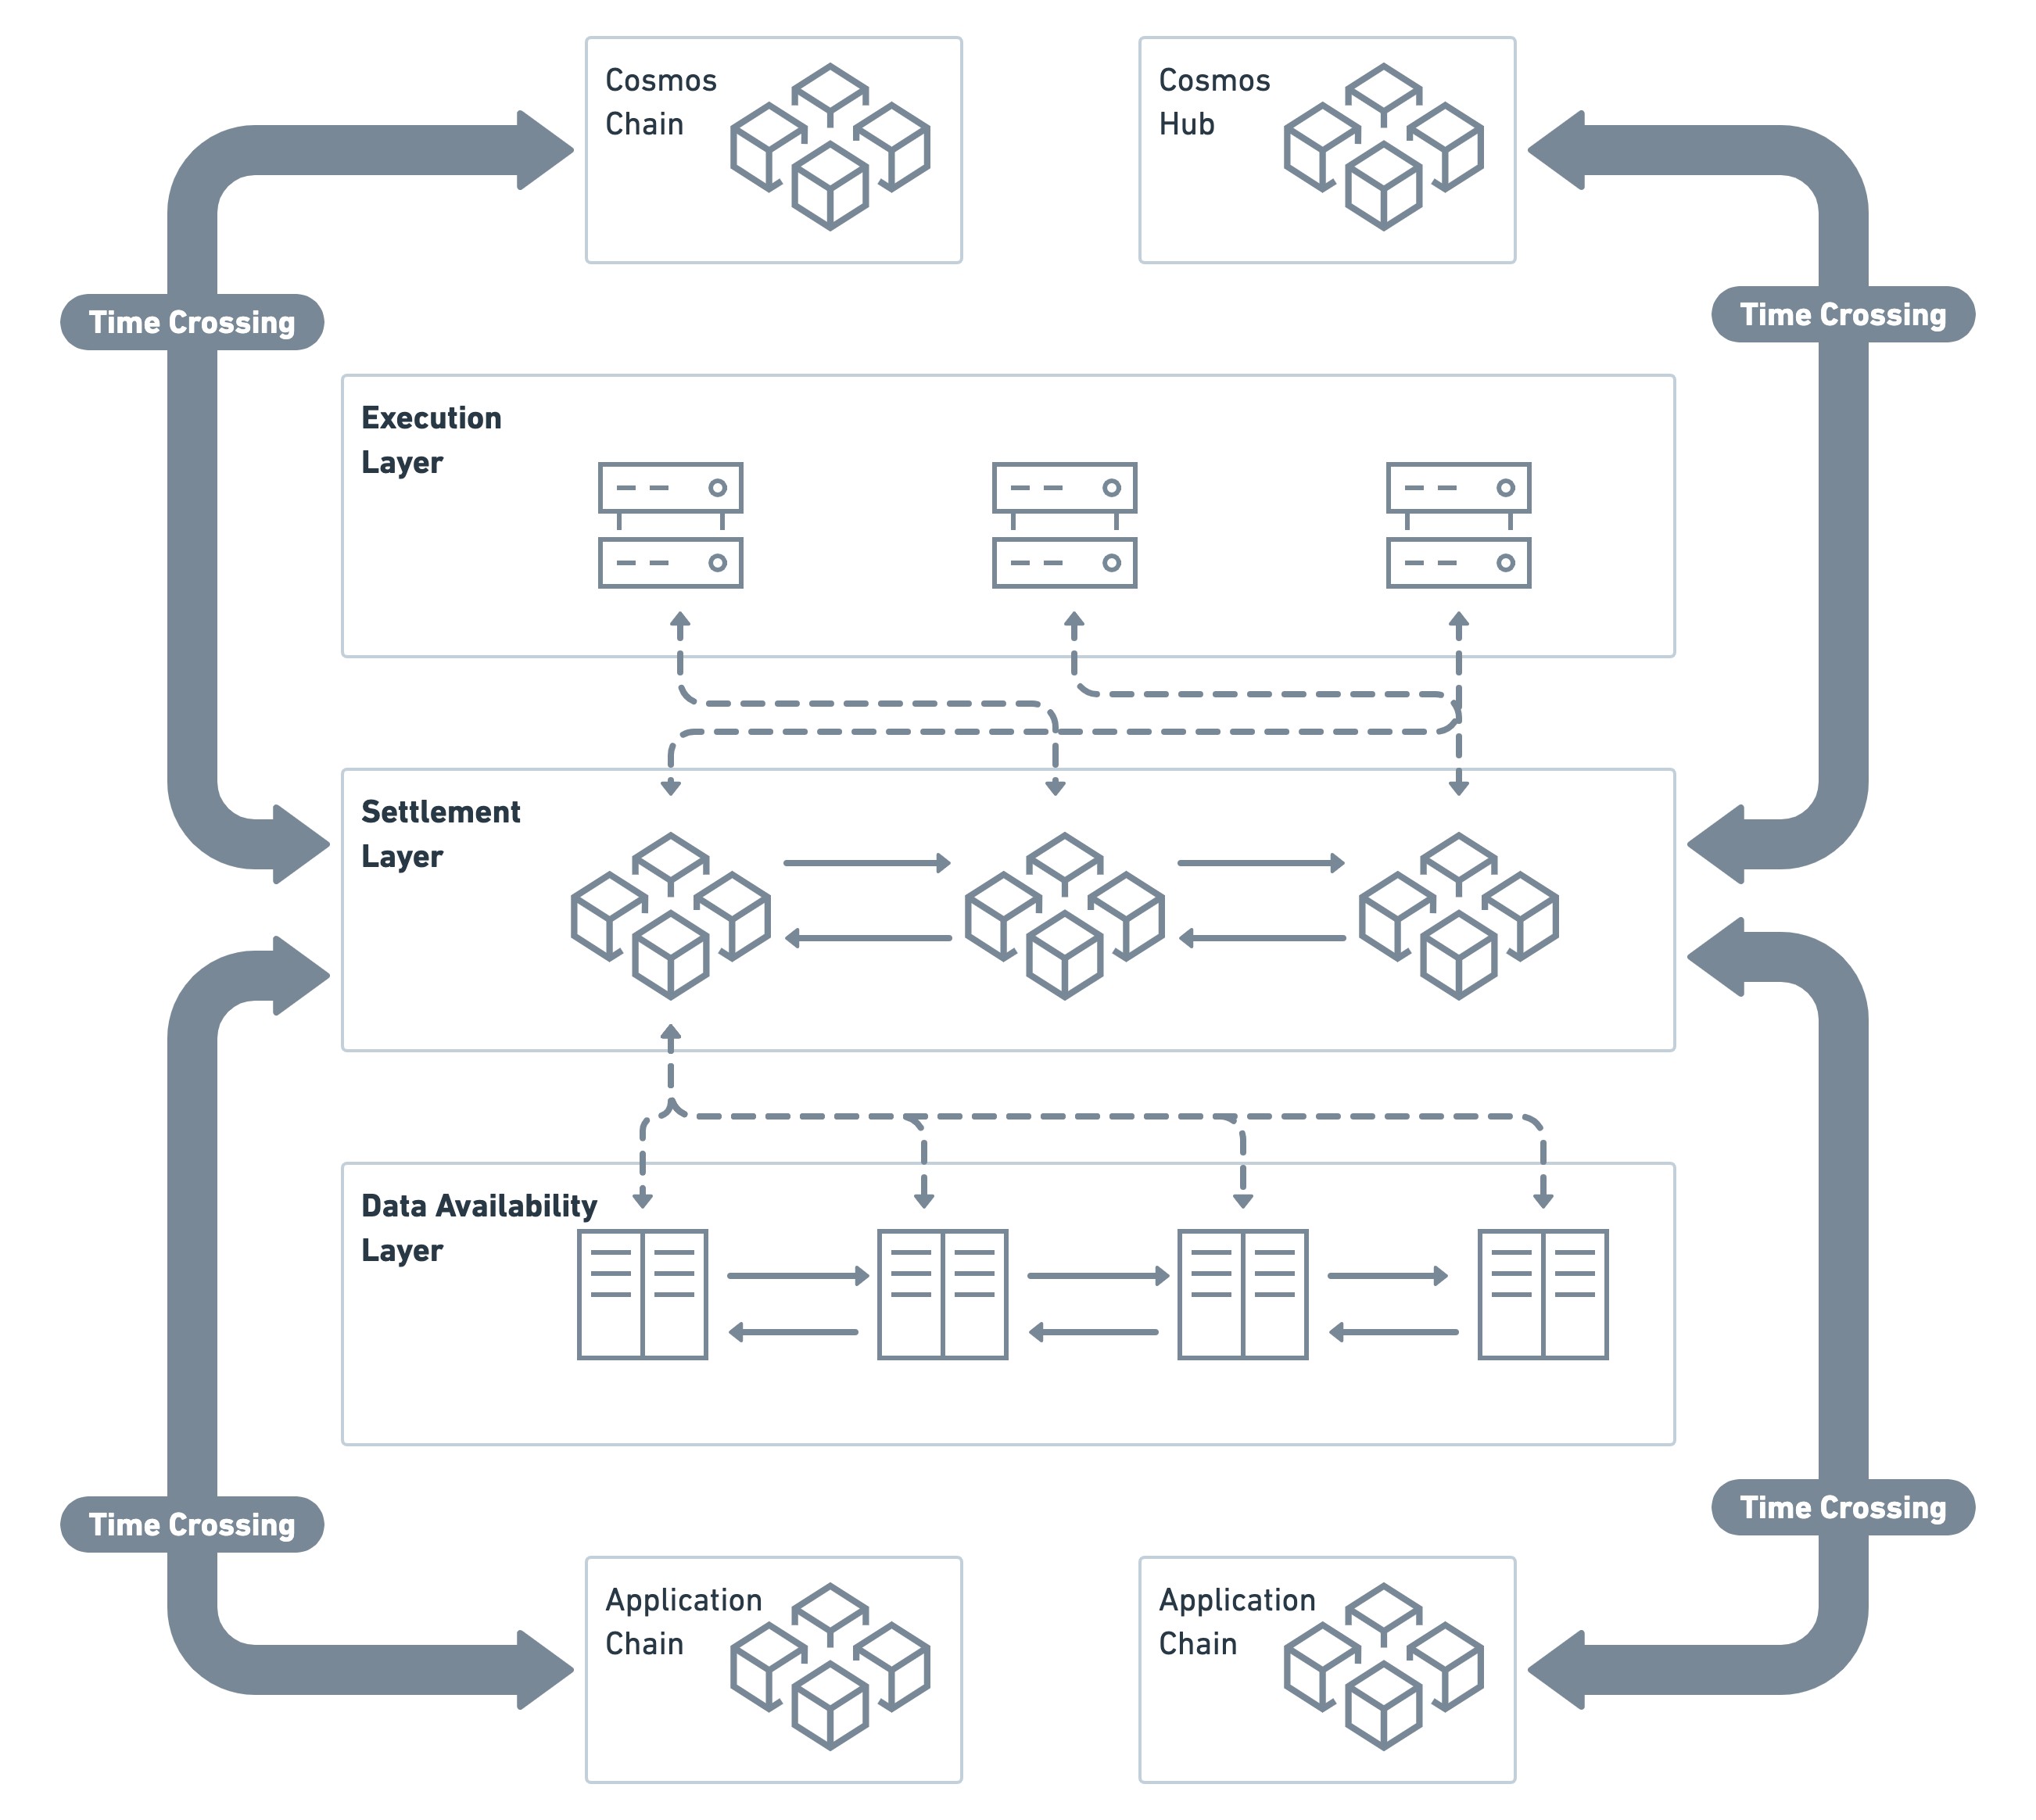
\includegraphics[width=0.8\textwidth]{images/1.png}
	\caption{\texttt{Cube} Architecture Diagram}
	\label{fig:1} 
\end{figure}

\subsection{Execution Layer: Built-in Rollup High-speed Execution Engine}
The execution layer is key to \texttt{Cube}'s scalability. \texttt{Cube} achieves scalability by offloading the expensive transaction process from on-chain to off-chain, while keeping its on-chain focus on validating the results. 

\texttt{Cube} uses Rollup technology as the main implementation of the execution engine, splitting the transaction process into two parts. The first is through combining a large number of transactions executed off-chain, and the second is to submit them as one to the main chain for validation. The original data of the transactions is packed and stored on the chain.This reduces the amount of data being sent to the main chain and enables faster and cheaper transactions and hundreds of thousands of TPS. 

\subsubsection{Rollup Technology Solution}
Rollup technology mainly includes ZK Rollup and Optimistic Rollup, which are currently the most mainstream Layer 2 scaling solutions for Ethereum. Both of them have different advantages and limitations in the current application scenarios. 

For Optimistic Rollup, it is fully compatible with EVM so it is very convenient for existing Ethereum Dapps to complete the migration, but it relies on a long waiting period for the transaction validation, and on-chain transactions take a long time to be confirmed.

For ZK Rollup, its security model relies on zero-knowledge proof of cryptography, andon-chain confirmation of transactions can be completed as long as the relevant zero-knowledge proof is verified However, due to the complexity of the zero-knowledge proof technology, a fully universal and reliable zkEVM is not yet available. This leads to each application having to develop its own zero-knowledge proof logic, making the development and migration of applications much more difficult.

\texttt{Cube} considers fast transaction validation critical and therefore prefers ZK Rollup as our execution layer. \texttt{Cube} will provide a ZK-Rollup SDK that integrates the zero-knowledge proof generation and verification process components. \texttt{Cube} has built-in templates for common applications, including DEX and Lending, making it easier for developers to integrate these capabilities.

In addition, \texttt{Cube} has proposed its own Collaborative Rollup that is fully EVM-compatible. It also offers fast transaction validation, aiming to provide a good alternative to ZK Rollup until the zkEVM technology matures.


\subsubsection{Data Availability Separation}
During the transaction execution, \texttt{Cube} only submits the results of the Rollup transactions to the settlement layer instead of submitting the raw transactions to the settlement layer like traditional Rollups. Before the results of the Rollup transactions can be submitted to the settlement layer they must be submitted to \texttt{Cube}'s data availability layer first. \texttt{Cube}'s data availability layer meets economic and data storage requirements, thus saving valuable storage resources on the settlement layer, as shown in figure \ref{fig:2}. 

After the transaction set is submitted to the data availability layer and confirmed, the data availability layer then sends back the proof of the availability corresponding to the Merkle tree root of the current transaction set.

For Collaborative Rollup, this proof of availability can be “rolled up” with the transaction result endorsement and submitted to the main chain. For ZK Rollup, the proof of availability is submitted to the chain along with the zero-knowledge proof, and this supports the Validium model of ZK Rollup.

\begin{figure}[h]
	\centering
	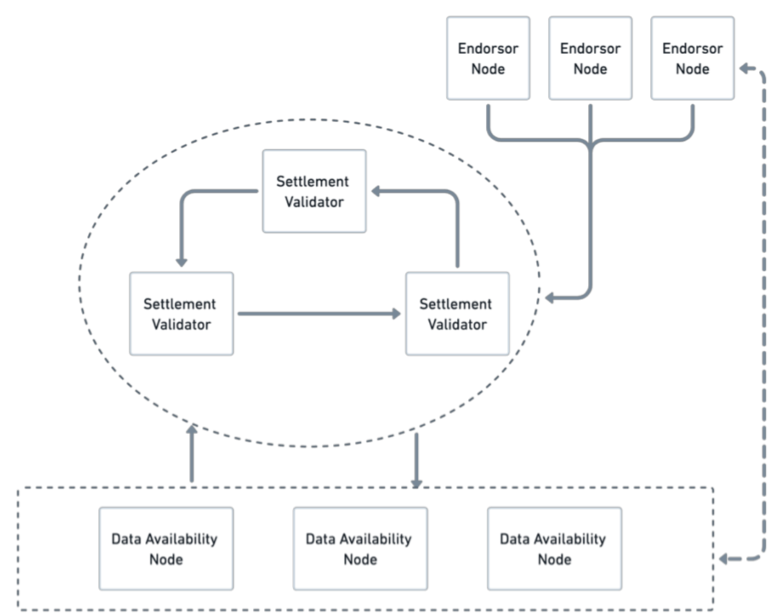
\includegraphics[width=0.8 \textwidth]{images/2.png}
	\caption{Separation of data availability at the settlement layer}
	\label{fig:2} 
\end{figure}


\subsection{Settlement Layer: the Highest Performance EVM-compatible Chain}
The settlement layer is the core of the \texttt{Cube}. For the execution layer, the settlement layer is the key to transaction fee and transaction confirmation. For the data availability layer, it is even more important, as the entire process of block construction, proposal, confirmation and transaction payment, are all driven by the settlement layer. 

At the same time, the settlement layer is also responsible for cross-chain functions. Assets from both application chains and other ecosystems flow into the \texttt{Cube} through the settlement layer. The \texttt{Cube} settlement layer is developed from Ethereum but with completely redesigned and optimized consensus and storage features, making it the highest-performing EVM-compatible chain today.


\subsubsection{Full Ethereum Protocol Compatibility}
\texttt{Cube} believes that Ethereum is the industry standard for blockchain applications development. To attract more high-quality Dapps projects and developers to join the \texttt{Cube} ecosystem, \texttt{Cube} has implemented the full Ethereum protocol in the settlement layer. 

The virtual machine \texttt{Cube} is not only fully compatible with EVM, but also keeps up with the latest EIP's so that developers can directly deploy the existing Dapps on Ethereum to \texttt{Cube}. All the development tools developed on Ethereum, including Wallet, Solidity, Remix, Truffle and Hathat, can also be directly used on the \texttt{Cube} Chain.

\texttt{Cube} is also compatible with almost all of the RPC interfaces of Ethereum, so developers can switch to \texttt{Cube}'s application development at no cost and get the rewards for \texttt{Cube}'s ecosystem development.


\subsubsection{Deep Performance-based Optimisation}
\texttt{Cube}'s approach to performance optimization begins with the settlement layer. While it is not responsible for executing specific user transactions, the settlement layer provides an anchor and foundation for the entire system. 

For this reason, \texttt{Cube} has developed its own combined DPOS and random sampling validator selection consensus mechanism, and a Pipelined Optimized BFT process to achieve extremely high performance, true decentralization, and an excellent balance of transaction throughput and instant confirmation. In addition, \texttt{Cube} has modified a storage synchronization and EVM execution cache based on EVM real-world actual performance profiling, resulting in significant performance improvements.


\subsection{Data Availability Layer: Massive Validators \& Unlimited Scalability}
To save the valuable storage space in the settlement layer, \texttt{Cube} designed the data availability layer to provide reliable on-chain storage for Rollup and various decentralized applications. This allows the original transaction data corresponding to rollup and the actual material corresponding to NFT do not need to rely on external storage protocols anymore. It can be completely solved inside the \texttt{Cube} Chain.

In addition, \texttt{Cube} has designed the data availability layer with a Sharding architecture to involve more nodes for increased decentralization and scalability. This allows a single node to store only a chunk of data (shard) while a large number of nodes ensures data availability. This solves the fundamental problem of increasing the number of nodes in a blockchain without increasing storage capacity.

As a separate storage layer, \texttt{Cube}'s data availability layer has the following main features compared to traditional blockchains:
\begin{itemize}
	\item[$\bullet$] Only data needs to be stored on the chain, no transaction needs to be executed, also there is no world state;
	\item[$\bullet$] Verification of a block does not rely on historical data;
	\item[$\bullet$] Only the settlement layer conducts unified management.
\end{itemize}


\subsection{Cross-Chain: Full Interoperability of Assets and Messages}
\texttt{Cube} is based on a cross-chain protocol that allows assets to flow in different dimensions. 

\texttt{Cube}'s cross-chain protocol is compatible with Cosmos IBC, making it easy to integrate into the Cosmos ecosystem. At the same time, it supports not only cross-chain transfer of assets but also cross-chain communication at the message level, laying the foundation for multi-application chain structures and cross-chain calls between DeFi's protocols.

In order to bridge the flow of assets between \texttt{Cube} and any other chain, \texttt{Cube} has built an Oracle-based cross-chain bridge as a complement to the cross-chain communication protocol when it is not applicable.


\section{Collaborative Rollup}
\texttt{Cube} introduces collaborative rollup as an execution engine.

\subsection{Security Model}
Unlike the security of ZK Rollup, which relies on cryptographic algorithms, the security model of Collaborative Rollup relies on the endorsement of a random group of verifiers, which is the origin of the term collaborative. \texttt{Cube} believes that a single verifier cannot be trusted, but a randomly selected group of sufficient verifiers can be. This security model is consistent with the security assumptions of Polkadot and Ethereum 2.0. 

Therefore, if the execution result of a transaction can receive the endorsement of more than half of a randomly selected group of verifiers, we can consider the execution result of the transaction to be trustworthy.

In addition, we establish a penalty mechanism for the case when a validator is found to endorse an invalid transaction result. After any validator submits the malicious endorsement to the chain as evidence of malicious behavior, the malicious validator will lose his stakes and a part of the stakes will be rewarded to the validator who was the first to submit the evidence.


\subsection{Node Classification}
Collaborative Rollup is divided into two roles in terms of protocol - one is an execution node and the other is an endorsement node.

The execution node is essentially a high-performance, centralized EVM that works on Layer 2 and keeps all the accounts and states of Layer 2. It needs to have an account on the settlement layer and stake. It is used for fast and efficient execution of the transactions and encapsulation of the execution results into an endorsement request that is sent to the endorsement nodes.

The endorsement node is also the full node of the execution layer. If the stake of a validator is more than a certain proportion, and he has registered in a specific system contract, he can become a candidate for an endorsement node. In the registration process you'll need to register two public keys. One is a property related public key to protect your belongings, the other is an endorsement related public key to sign an endorsement.

Then each epoch endorsement node-set will be randomly selected from these candidate endorsement nodes. There can be a fixed number of sets of the endorsement nodes, and the number of endorsement nodes in each set is constant.


\subsection{Validation and Endorsement}
As mentioned above, the execution nodes need to pack the transactions of the execution layer and execute them. After each transaction is executed, changes will be made to the current world state.

Like ZK Rollup, Collaborative Rollup also uses the shortened version of the addresses and forms all states into a Merkle tree structure. The Collaborative Rollup adopts the MPT of Ethereum, so that we can use the root of this tree to represent the current world state of Rollup and can get Merkle proofs for specific states.
With the above execution environment, we can define below how to represent the execution result of a transaction. To achieve separation of execution and verification, the execution result must be verifiable. We define the execution result as follows.

As shown in the figure \ref{fig:3} above it contains the following main components.
\begin{itemize}	
	\item[$\bullet$] The Merkle tree consists of the original set of transactions and its root $root_{tx}$;
	\item[$\bullet$] The state root before transaction execution $root_{pre-state}$;
	\item[$\bullet$] The post-transaction execution state $root_{post-state}$;
	\item[$\bullet$] The read-set and write-set associated with transaction execution and the corresponding Merkle proof for $root_{pre-state}$;
	\item[$\bullet$] Execution node signature.
\end{itemize}

\begin{figure}[!htbp]
	\centering
	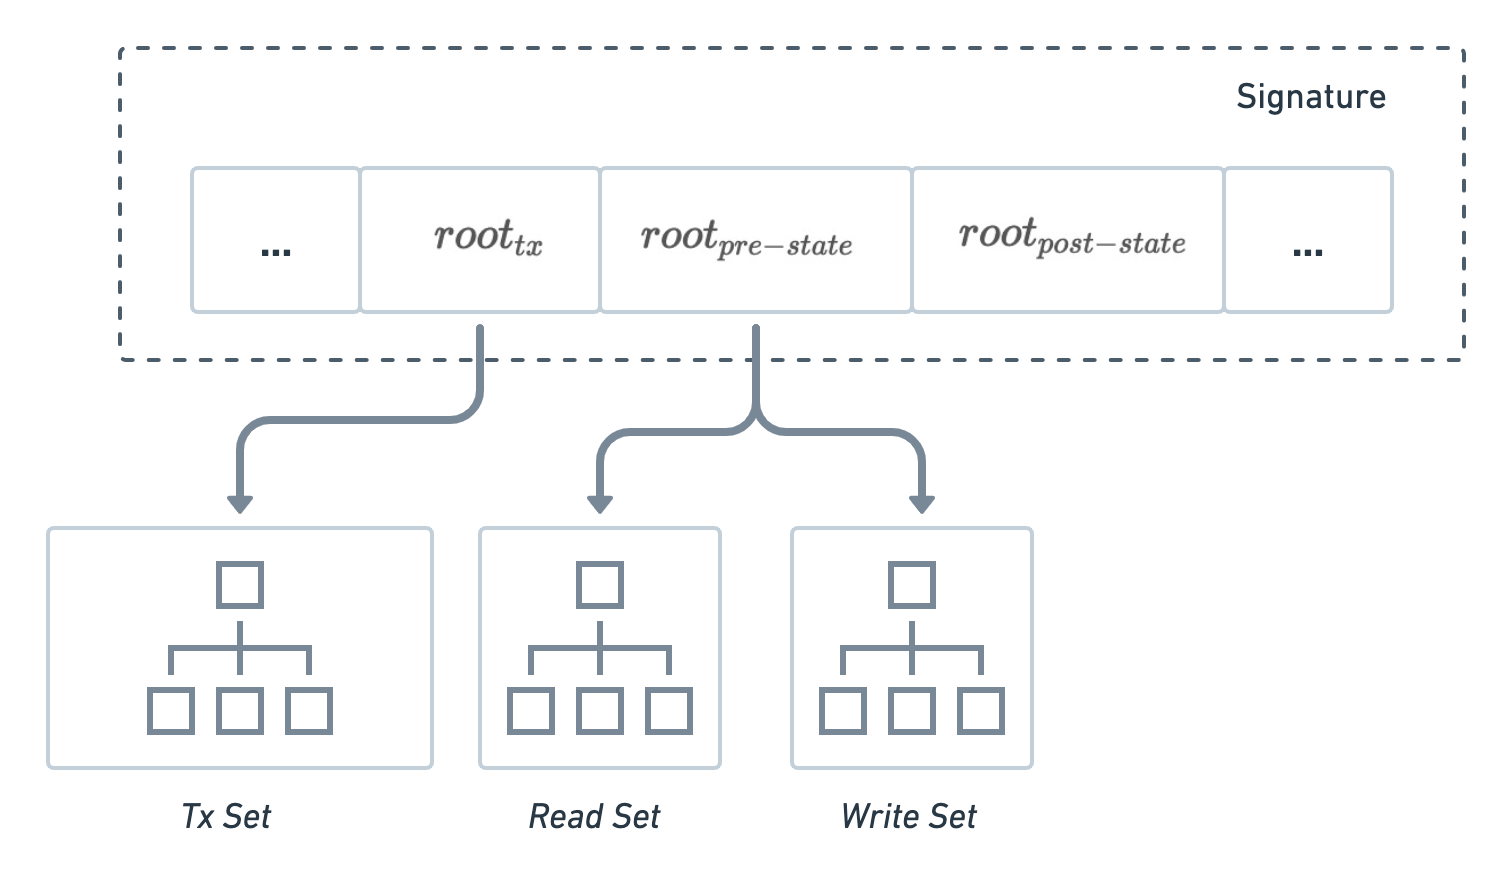
\includegraphics[width=0.8 \textwidth]{images/3.png}
	\caption{Transaction execution results}
	\label{fig:3} 
\end{figure}

As is shown in the figure \ref{fig:4}, after receiving the endorsement request, the endorsing node will first verify the signature, and the sender's identity by its stake amount. Then verify the corresponding Merkle branches of the read-set and write-set, and execute the transactions in EVM with the read-set to get output values of the write-set, and most of all combine the write-set with its Merkle branches before execution to update the state tree root. It also verifies whether the final state root obtained at the end is consistent with the one after execution in the endorsement request. If the above verification is passed, then the BLS private key is used to sign all the parts except the original transaction set, which is the endorsement of the execution result of this batch of transactions. 


\begin{figure}[!htbp]
	\centering
	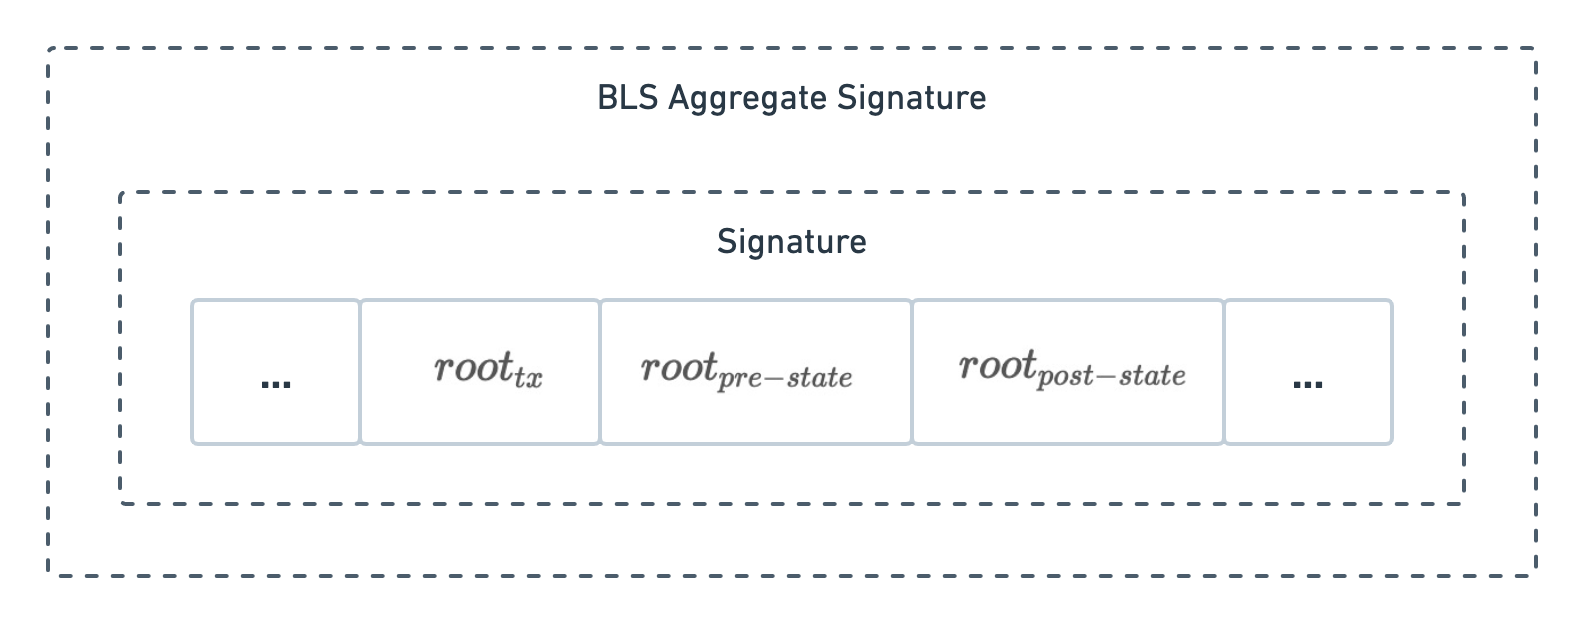
\includegraphics[width=0.8 \textwidth]{images/4.png}
	\caption{Endorsement of transaction execution results}
	\label{fig:4} 
\end{figure}


\subsection{Transaction Execution Flow}
As mentioned above, when a node becomes an execution node and an endorsement node by staking tokens, the endorsement nodes are randomly divided into multiple groups at each epoch. After that Collaborative Rollup transaction processing can be performed in the figure \ref{fig:5}, 

First, the execution node is responsible for receiving transactions from clients, and after executing a batch of transactions, it packs the execution result as an endorsement request in the way described above. Then, the endorsement request is broadcasted to the corresponding set of endorsing nodes in the current epoch. After the endorsing node finishes verifying the transaction, if the transaction result is valid, it will broadcast the transaction after endorsing it and collect the endorsement of the current set of endorsing nodes for this transaction. When an endorsing node collects more than half of the transaction endorsements, it aggregates the signatures and broadcasts them together with the endorsement contents to the settlement layer. At the same time, the execution node itself can also collect the aggregated endorsements and send them to the settlement layer. After verifying the aggregated signatures, the settlement layer updates the chain status and completes the deduction of transaction payments and all endorsing nodes are rewarded with transaction fees.

\begin{figure}[!htbp]
	\centering
	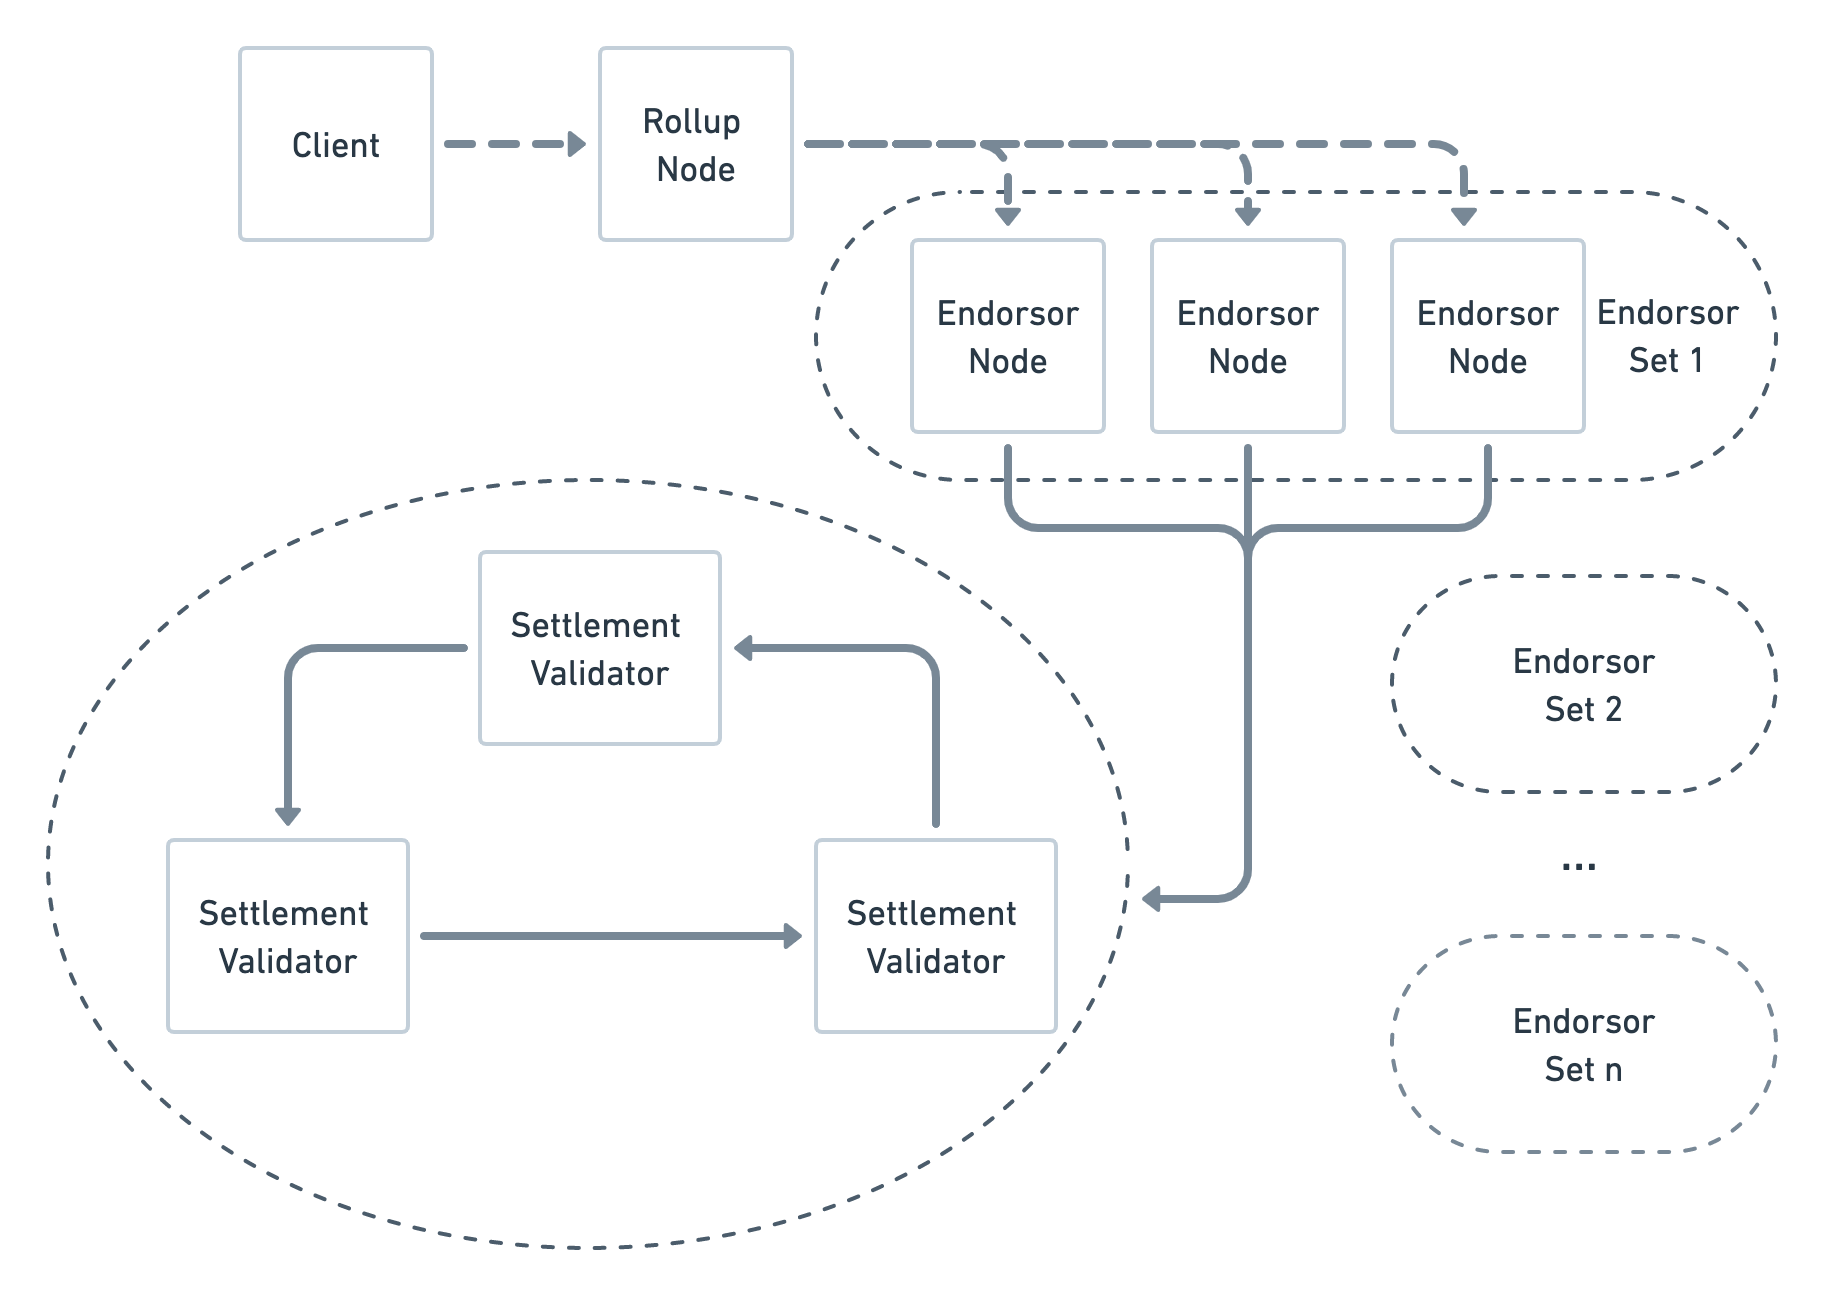
\includegraphics[width=0.8 \textwidth]{images/5.png}
	\caption{Collaborative Rollup transaction execution}
	\label{fig:5} 
\end{figure}

If during the verification process an endorsing node finds a transaction is invalid, it can also mark the transaction as invalid and then endorse it. After collecting enough endorsed transactions, these endorsements can also be aggregated and sent to the settlement layer, then the only invalid transaction will be fined without changing the on-chain state. Through this mechanism we avoid the situation when execution nodes intentionally send invalid transactions for endorsement, which could result in a waste of computing resources of the endorsing nodes.

In addition, since each endorsing node verifies the transaction results, it is very easy to detect malicious behavior of other endorsing nodes, including:

\begin{itemize}
	\item[$\bullet$] Endorsing invalid transaction results;
	\item[$\bullet$] Marking valid transactions as invalid and endorsing them.
\end{itemize}

If an endorsement node finds malicious behavior mentioned above it can submit it as evidence to the chain, then the malicious endorsement node's stake will be slashed, and the node that submits evidence can receive a reward.


\section{Chaos Consensus}
Consensus is the core components of blockchain, and \texttt{Cube} uses a hybrid randomized DPOS protocol, which we named “Chaos Consensus”. This protocol is based on the DPOS consensus and introduces a random selection mechanism for nodes, which allows more nodes to participate in the consensus and increases the decentralization of the system. The BFT consensus mechanism is used among the consensus nodes to provide the system with fast confirmation of transactions. In addition, the traditional consensus process is disassembled into separate transaction sequence consensus and execution result consensus, and together with the execution process, a pipeline mechanism is formed for transaction processing, which greatly improves the overall throughput of the system.


\subsection{Protocol Overview}
“Chaos” consensus is a protocol used to select the set of nodes to propose and validate blocks, which is an important mechanism to introduce more nodes into the system to participate in the consensus process. The consensus process is divided into different epochs according to a fixed number of blocks, and the same set of validators is used in one epoch for proposing and validating blocks.


\subsection{Validator Set Generation}

As with the usual DPOS protocol, any node can become a qualified validator by staking a certain amount of tokens to the system contract, and other users can stake their tokens to a trusted validator and become a delegator. The stakes of each validator are the sum of its own stakes and the delegation of other users.
The system then ranks the top 100 nodes according to the number of stakes by the validator and selects the set of candidate validators. The top 15 nodes directly become the active validators, and then the system randomly selects 6 active validators from the remaining 85 nodes based on a jointly generated random number, forming a set of 21 active validators. The newly selected active validators will come into effect in the next epoch. In addition, the number of candidate validators can be increased as the node size grows in the future.


\subsection{Random Number Generation Algorithm}
The generation of random numbers has to be done in a decentralized scheme, and it is also necessary that the generated random numbers are verifiable and that the random numbers generated by all nodes are guaranteed to be consistent. Moreover, in the process of generating random numbers, no single node can influence or even manipulate the generation of random numbers.

The random numbers of the \texttt{Cube} are generated in the MPC way, i.e., each participating node first generates its own random numbers locally, and then the system uses certain operations to generate a public random number based on the numbers generated by each node. In order to ensure that each node cannot know the random numbers of other nodes before generating its own random numbers, \texttt{Cube} uses the cryptographic PVSS (Publicly Verifiable Secret Sharing) scheme based on Shamir Secret Sharing in the random number generation process. This scheme allows the current set of validators to collectively generate a random number and uses cryptographic methods to ensure that no one can manipulate the random number generation process. Process is:
\begin{enumerate}
	\item[$\bullet$] Validator D divides its secret S into n pieces $(S_1,..., S_n)$ according to the threshold t: encrypt it according to the public keys $(P_x,..., P_N)$ of n participants respectively, generate the corresponding commitment (zero-knowledge proof), and share all of the information;
	\item[$\bullet$] Anyone can verify that the n value of D is valid without obtaining additional information;
	\item[$\bullet$] If necessary, participants can decrypt the share with their private key, and then share it with others;
	\item[$\bullet$] Anyone can reconstruct the secret RS after obtaining $\ge t$ decrypted shares, and $RS == S$.
\end{enumerate}


The generation of a common random number is performed at each epoch. The current epoch uses the random numbers generated by the previous epoch.


\subsection{Streamline Consensus}
In traditional blockchain systems such as Ethereum, the block generation process consists of several steps:
\begin{itemize}
	\item[$\bullet$] The miner (block proposer) packs the transaction and executes it;
	\item[$\bullet$] The miner set the execution results to the block header;
	\item[$\bullet$] Block propagation;
	\item[$\bullet$] Other nodes execute the transactions in the block;
	\item[$\bullet$] And then validate the execution results of the block.
\end{itemize}

It can be seen that a transaction undergoes two serial executions from the time it is packaged to the time it reaches network-wide consensus, in addition to a serial propagation process, which has a lot of room for optimization.
We take a closer look at the structure of a block, which contains a batch of transactions and various Merkle roots associated with the execution results.
The transaction list mainly represents the sequence of transaction execution, while the block header can be seen as the result of the block execution. We can consider separating the consensus of these two into a transaction sequence consensus and an execution result consensus.


\subsection{BFT Consensus Flow}
As shown in the figure \ref{fig:6}, assuming that the block for consensus is block $N$, the BFT does not consent to the entire block $N$, but the transaction list and some meta-data of block $N$, and the block hash of block $N-2$. After the BFT completes, the consensus on block $N+1$ continues, and block $N$ is executed at the same time. In addition, since block $N$ carries the hash of block $N-2$, the completion of consensus on block $N$ also means the completion of confirmation on block $N-2$.

\begin{figure}[!htbp]
	\centering
	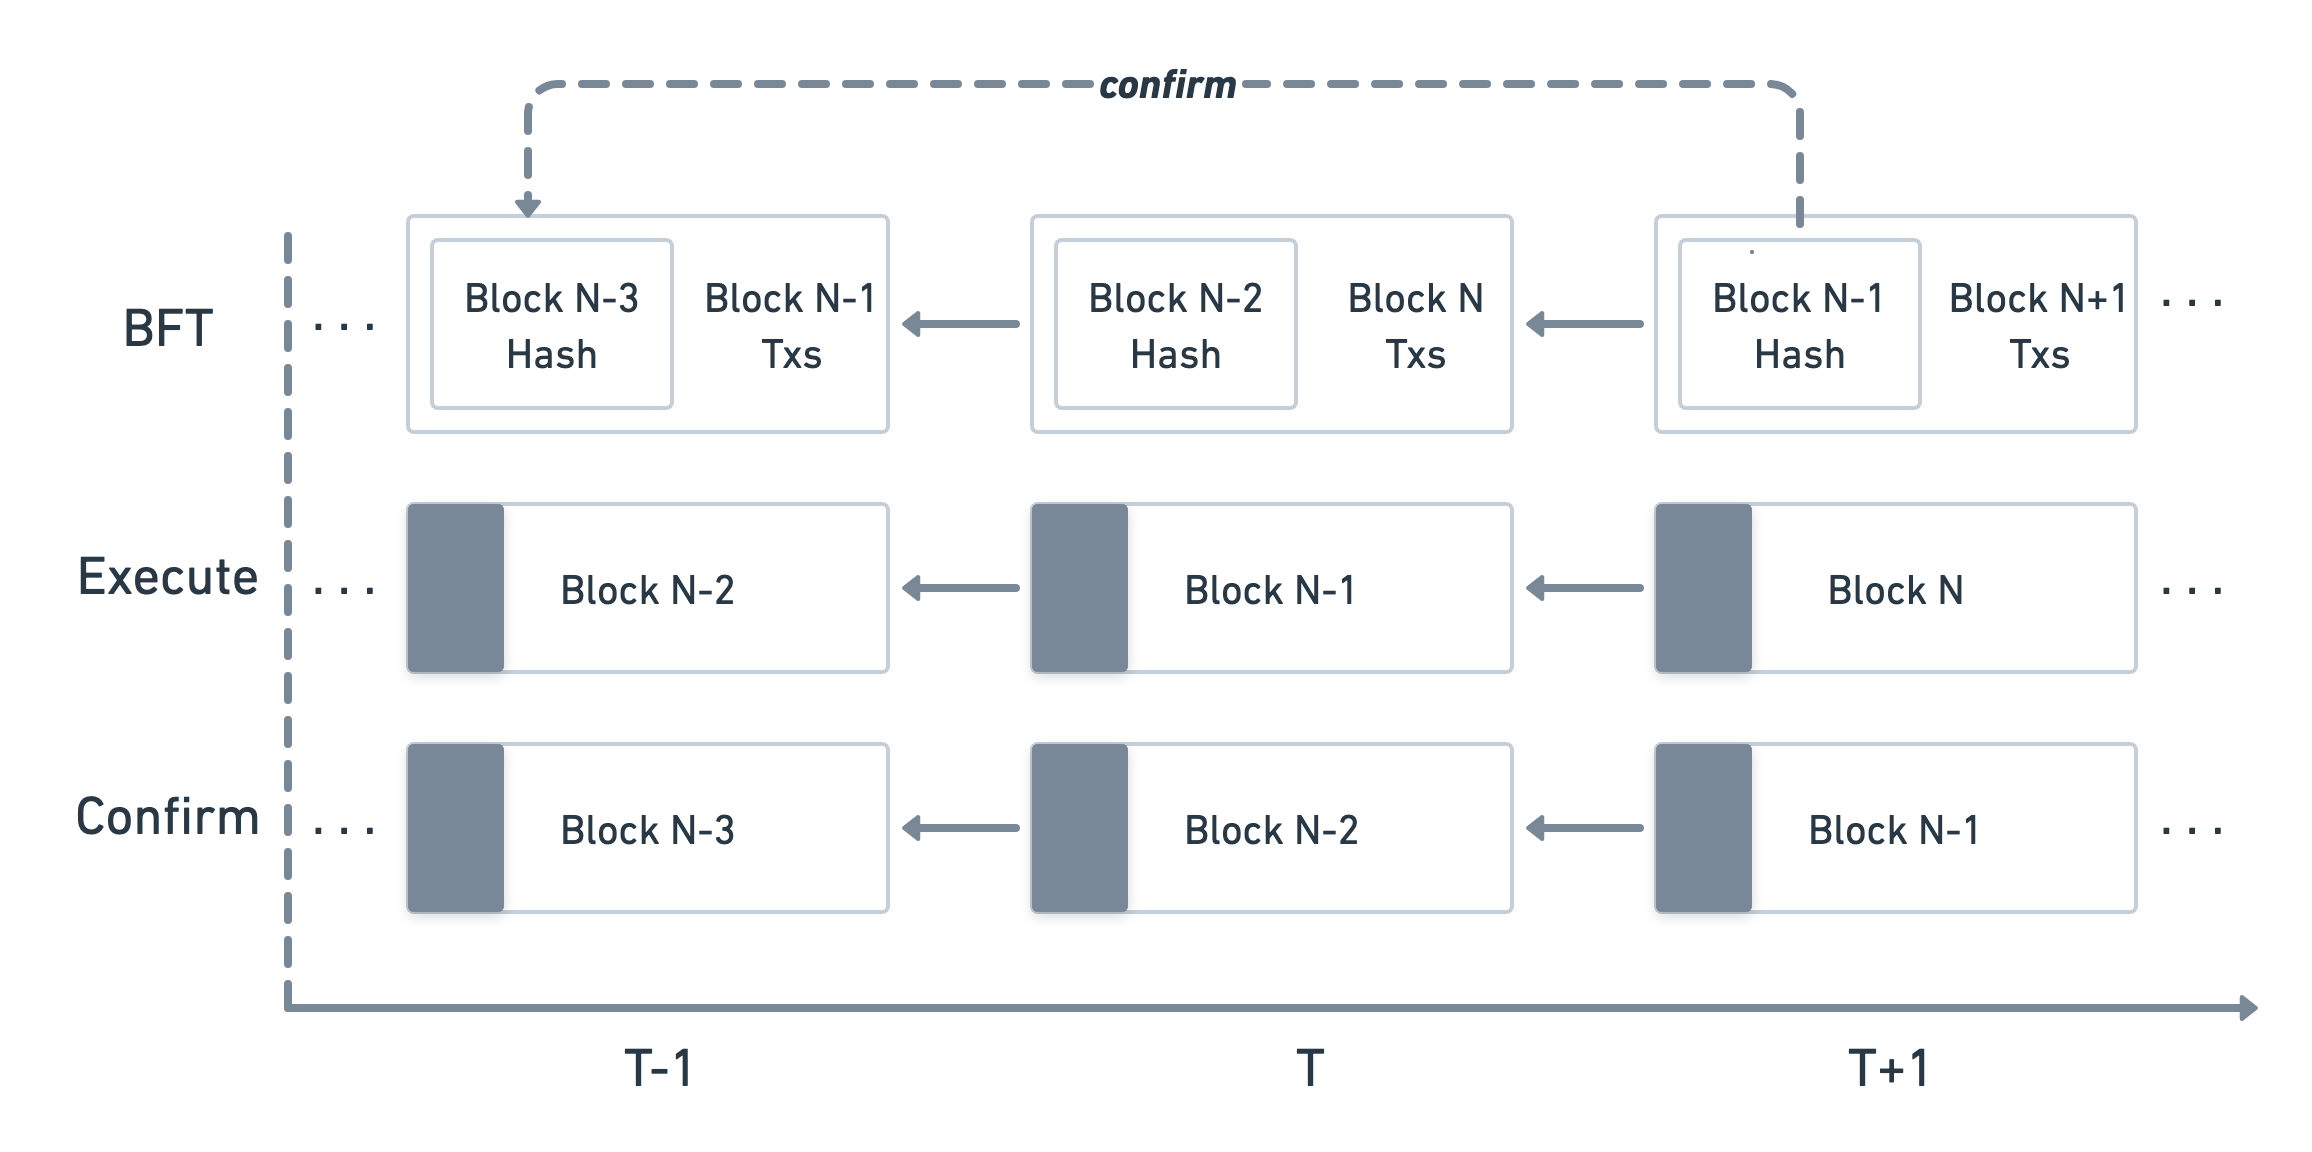
\includegraphics[width=0.8 \textwidth]{images/6.png}
	\caption{Pipelined processing of BFT, execution, and validation.}
	\label{fig:6} 
\end{figure}

\section{Data Availability Sharding}
\texttt{Cube} proposes a sharding mechanism based on block slicing, which splits a complete block into a fixed number of pieces (shards) according to the storage size with certain encoding rules. Each node can choose to store not only all the data, but also a fixed number of pieces in a verifiable random sampling. In either case, the current storage block can be verified, so that any node can become a verifying node by staking, allowing the whole system to achieve greater decentralization. Moreover, since the validation node does not need to store all the data, the overall capacity of the system increases with each node added, thus providing good scalability.

The operation and management of the data availability layer relies on the settlement layer, including the acceptance and payment of storage transactions, the packaging and proposal of integrated blocks of the data availability layer, and the final confirmation of this data availability layer block. In addition, the staking and management in the Data Availability Layer validation nodes also rely on the settlement layer.

Nodes are classified into the following types at the network level in figure \ref{fig:7}:
\begin{itemize}	
	\item[$\bullet$] Light nodes, which keep only the block header and can verify the availability of the block data through sampling to determine whether to accept the block header;
	\item[$\bullet$] A sampling node, which stores the block header and a partial sampling of the block and can validate the block;
	\item[$\bullet$] Full node, contains an entire copy of blockchain ledger verifies blocks and block's sharding, provides fraud-proof.
\end{itemize}


\begin{figure}[!htbp]
	\centering
	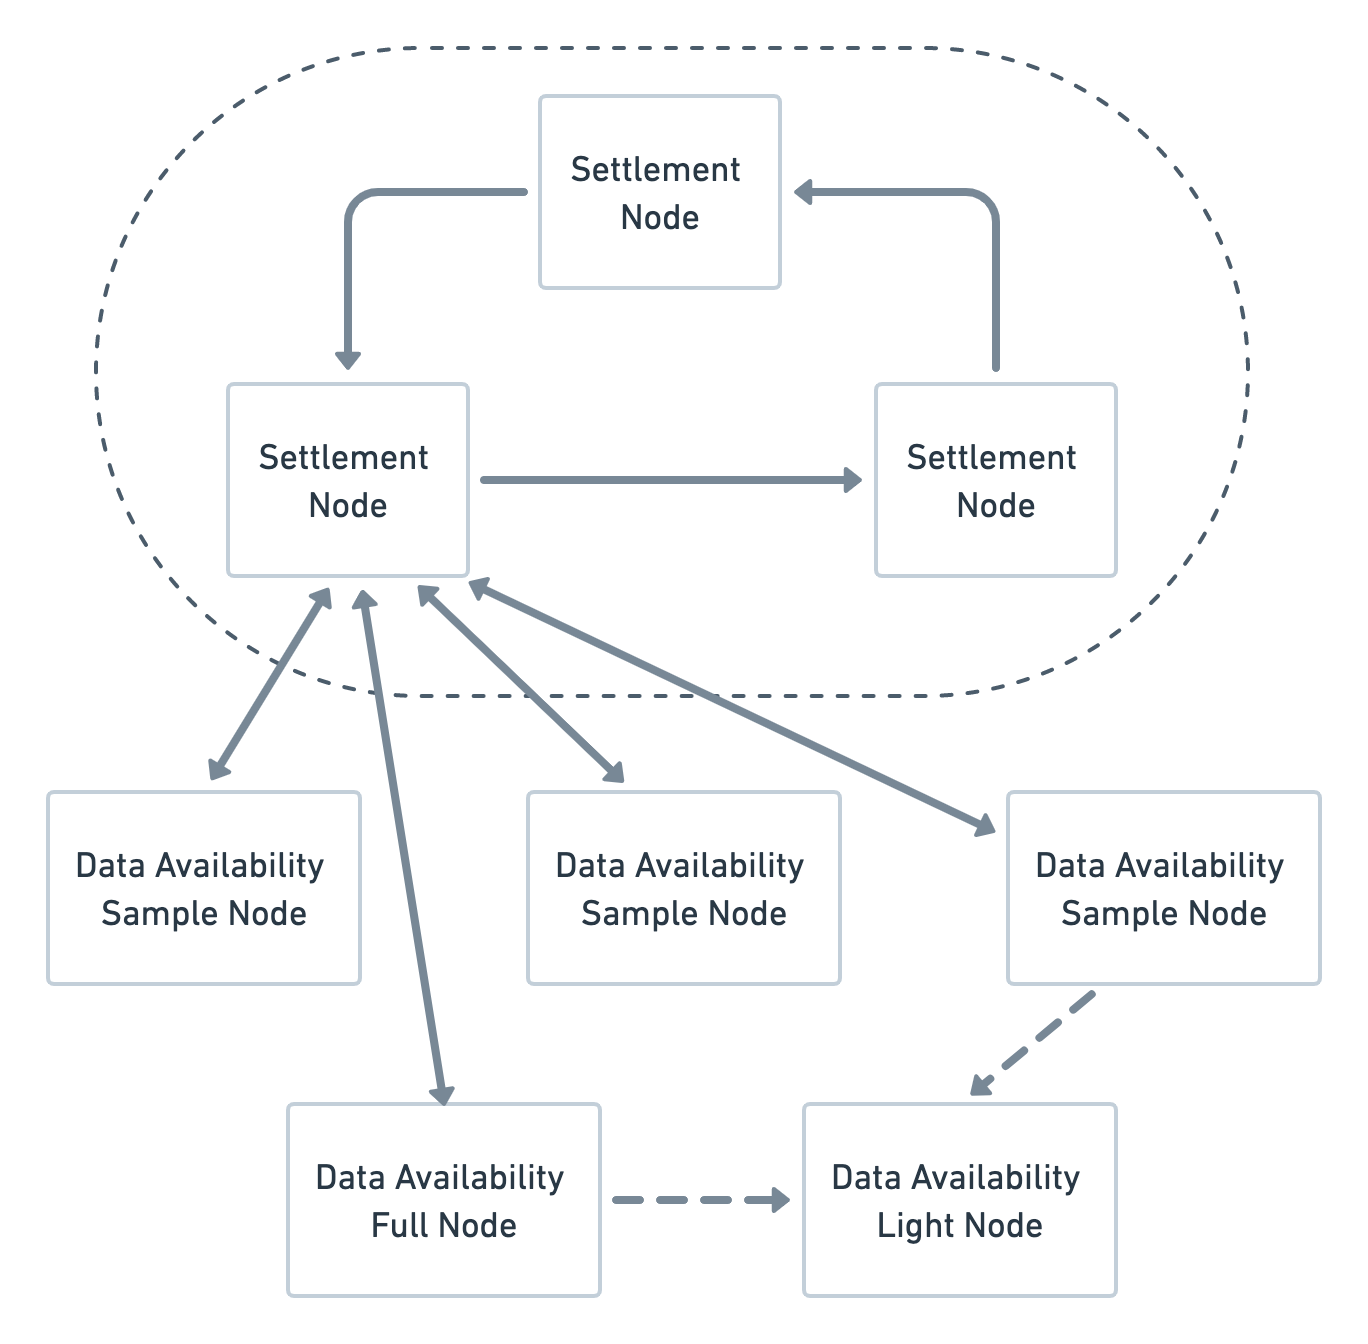
\includegraphics[width=0.7 \textwidth]{images/7.png}
	\caption{Data availability layer network architecture}
	\label{fig:7} 
\end{figure}



\subsection{Model and Assumptions}
Network model assumptions
\begin{itemize}
	\item[$\bullet$] Network topology assumptions: nodes are linked in a P2P way, and at least one of the network connections of each honest node is from an honest node;
	\item[$\bullet$] Network delay assumption: The maximum delay of the network is $D$. If an honest node obtains a certain data in the network at time $T$, other honest nodes can obtain the same data until the time of $T+D$.
\end{itemize}

Security assumptions
\begin{itemize}
	\item[$\bullet$] More than $2/3$ of honest nodes across the network;
	\item[$\bullet$] Honest storage nodes store sampled slices of all validated blocks.
\end{itemize}


\subsection{Proof of Data Availability}
Each transaction in the data availability layer is actually a request to store a piece of data that can be represented by its hash. The hash value of each transaction in the current block can form a Merkle tree, the root of which is stored in the block header as the data root of the current block. 
The Merkle path from the data hash of each transaction to the data root of the current block is the proof of availability of the data corresponding to the current data hash.


\subsection{Block Production Flow}
Since the protocol of the data availability layer does not need to validate transactions, but only the parent hash is required to generate blocks, both sampling nodes and full nodes can become validation nodes by staking a specific amount of tokens in the settlement layer and validate the blocks through random sampling. The generation and validation of blocks in the data availability layer are performed by the nodes in the settlement layer by submitting the evidence related to the data availability layer to the blockchain in the settlement layer.

First, the user broadcasts the storage transaction to the blockchain, and the current settlement layer node packs the valid storage transaction into a data availability layer block after the transaction is paid and verified, and then writes the storage paid transaction and the storage block hash to the settlement layer block, where the data availability layer block height and hash are written to the block header. The nodes in the data availability layer are all light nodes in the settlement layer, and the validation of the currently proposed block can be confirmed from the settlement layer block header. When the settlement layer block containing storage payment is executed, the storage fee will be deducted from the balance of storage transaction senders. But the fee will not be transferred to related accounts temporarily, thus locking the storage payment. 

In addition, the block body is the 2-dimension erasure code of the original data [1,3]. When a block is produced, it is sliced into $k * k$ pieces by size and then $2k * 2k$ pieces are generated by applying the 2-dimension RS (Reed-Solomon) code. Then the Merkle trees are created for each row and column of each fragment, so there are $2k + 2k = 4k$ Merkle trees, in the figure \ref{fig:8}.

\begin{figure}[h]
	\centering
	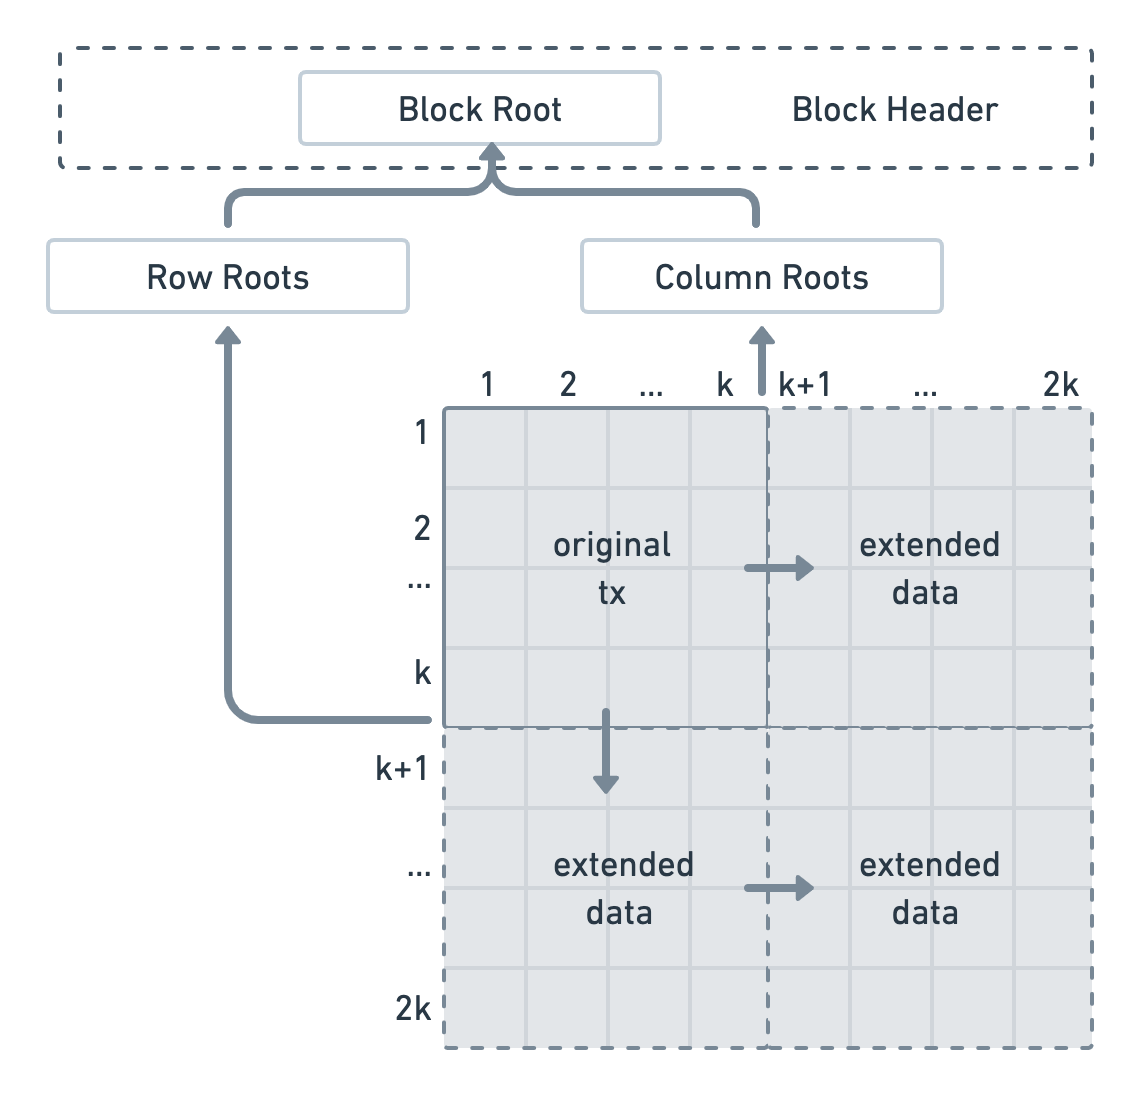
\includegraphics[width=0.7\textwidth]{images/8.png}
	\caption{Block slicing and encoding of data availability layer}
	\label{fig:8} 
\end{figure}

These 4k Merkle roots are finally formed into one Merkle tree, and the root of the tree is used as the root of the whole block. Then the slices are broadcasted in a P2P way, and for the full node all slices will be collected and restored and fraud proofs will be generated for blocks that cannot be restored. For the sampling nodes, slices are randomly selected for sampling according to a specific algorithm. When the sampling is completed, a random sampling certificate is generated and it will be signed and broadcasted afterwards to the settlement layer.

The settlement layer nodes collect the first c randomly sampled proofs that pass the verification and then apply the zero-knowledge proof technology to compress them into a single proof and submit it to the chain with the height, hash, and data root of the current storage block as a transaction. After the settlement layer miner verifies the proof and waits for $2D$ time after the data availability layer block is proposed, and no relevant fraud-proof is found, the data availability layer block is considered valid and the above transaction is packed into the next block. Then the related rewards will be distributed to the settlement layer node of block proposing, storage nodes of providing selected sampling proof and settlement layer node of submitting confirmation proof. The rewards come from the deducted storage payments described above. 

If, after $4D$ time, if enough proofs cannot be received from the data availability layer or fraud-proof is received from full nodes, the block height will be null and the previous storage fee will be returned. For the scenario with fraud proofs, all staking amounts and rewards of the nodes in the settlement layer of the proposed storage block will be slashed, and the full node in the data availability layer that provides the fraud proofs and the node in the settlement layer that packages the fraud proofs receive the rewards.

The remaining data availability layer nodes obtain the current status of the data availability layer blocks by synchronizing the settlement layer block header state.


\subsection{Random Sampling Proofs Based on zero-Knowledge Proofs}
After the sampling node has completed verifying the availability of the block, it needs to sign the sampling results and send them to the settlement layer nodes. After the settlement layer receives enough successful sampling results, it needs to pack them together into the next block and pass those over to other settlement layer nodes for verification.

This requires the sampling node to provide proof of sampling, which able to 
\begin{itemize}
	\item[$\bullet$] Prove to the settlement layer node that it has performed the required number of samples;
	\item[$\bullet$] Prove to the settlement layer that the pieces it sampled were chosen randomly in certain rules, i.e., the randomness can be verified;
	\item[$\bullet$] Multiple sampling proofs can be aggregated into a small proof which can be verified quickly.
\end{itemize}

For the first two requirements, consider the following structure
\begin{itemize}
	\item[$\bullet$] Block header of the DA layer contains block number, block hash, Merkle root of all fragments;
	\item[$\bullet$] Proofs of all Merkle sampling segments;
	\item[$\bullet$] Signatures for the above data.
\end{itemize}

In order to ensure that all sampling nodes can perform random sampling, Instead of taking the first few fragments as their own sampling results, we need to verify the randomness of the sampling. Consider a random number generator, and the random number is seeded by the hash of the current block combined with the public key of the node, i.e.,
$$seed = sha256(hash_{block} + publicKey)$$

In this way we can force the node to perform sample slicing corresponding to the first random numbers generated by this random number generator, so that the entire block slice is sampled uniformly in general, thus ensuring the data availability of the block.
The verification of the random sampling proof is as follows
\begin{itemize}
	\item[$\bullet$] Verify that the block header is proposed by the settlement layer;
	\item[$\bullet$] Verify the signature to ensure that this proof is generated by the staking node;
	\item[$\bullet$] Generate the index of the random sample according to rules above and verify that there is a sampling atindex position;
	\item[$\bullet$] Verify the Merkle proof of sampling.
\end{itemize}


Consider the third requirement above. Because the large number of random sampling proofs have to be collected (around 100), it requires a method to compress these proofs for faster verification. Consider the combination of proofs of availability and zero-knowledge proofs. The above verification process can be expressed as a zero-knowledge proof circuit system, where the hash of the verified block and the set of public keys of the sampling nodes are public parameters and the set of sampling proofs are so-called private parameters so that the produced proofs can be small enough to perform fast verification.


\subsection{Fraud-Proof}
The availability sampling of the above blocks only ensures that there are enough slices (shards) in the network to recover the corresponding blocks. However, some of the data in these slices might be invalid, and hence solving the above problem by fraud-proof is necessary. 

Fraud proof can be divided into proof of invalid transaction as well as proof of invalid data encoding, and for the storage chain only the latter needs to be focused on.
The generation of fraud-proof relies on all the data, so it requires full nodes or a sampling node that collects all the slices (shards) to generate it.

When these nodes collect enough fragments but cannot decode them correctly, they need to broadcast these fragments and their Merkle proofs, which are the so-called fraud-proof, then other nodes can verify them accordingly. The first submitted fraud-proof node will be rewarded.


\section{Time Crossing Protocol}
\texttt{Cube} believes that the future will be a world of interconnected chains. This is why \texttt{Cube} has designed and developed the “Time Crossing” cross-chain communication protocol to facilitate collaboration with assets from multiple ecosystems. In addition, \texttt{Cube} has built a multi-chain structured network on top of the cross-chain communication protocols to effectively meet the needs of application chains.


\subsection{Cross-chain Validation}
The key to cross-chain communication is how the target chain can effectively verify the cross-chain messages sent by the source chain, and the Time Crossing cross-chain protocol enables a decentralized, trustless way of cross-chain verification. To achieve this we need to establish a root of trust between the two parties of the cross-chain. When establishing a cross-chain relationship, both parties need to register the genesis block header into the other chain. The block header contains valid consensus proof of the current block. Therefore, the block header of the genesis block is the trusted root of both parties.

After that, both parties of the chains use it as the starting point to synchronize all subsequent block headers in real-time, which means the relationship between the two is equivalent to a mutual light node. Since the block header contains the set of valid validators in the next time period, by tracing the block header, we can confirm the valid validators set of each other's blockchain, thus confirming the validity of all subsequent blocks by following the block headers.

Once both sides of the chains have a mutually trusted block header, the verification of cross-chain messages can be achieved. \texttt{Cube} includes Merkle proofs of these state changes when sending cross-chain messages. The other blockchain can use these Merkle proofs to verify the validation of these state changes when verifying the messages and decide whether to perform the corresponding operations on its side. This enables automatic and decentralized cross-chain operations between the two blockchains, as in the figure \ref{fig:9}.

\begin{figure}[!htbp]
	\centering
	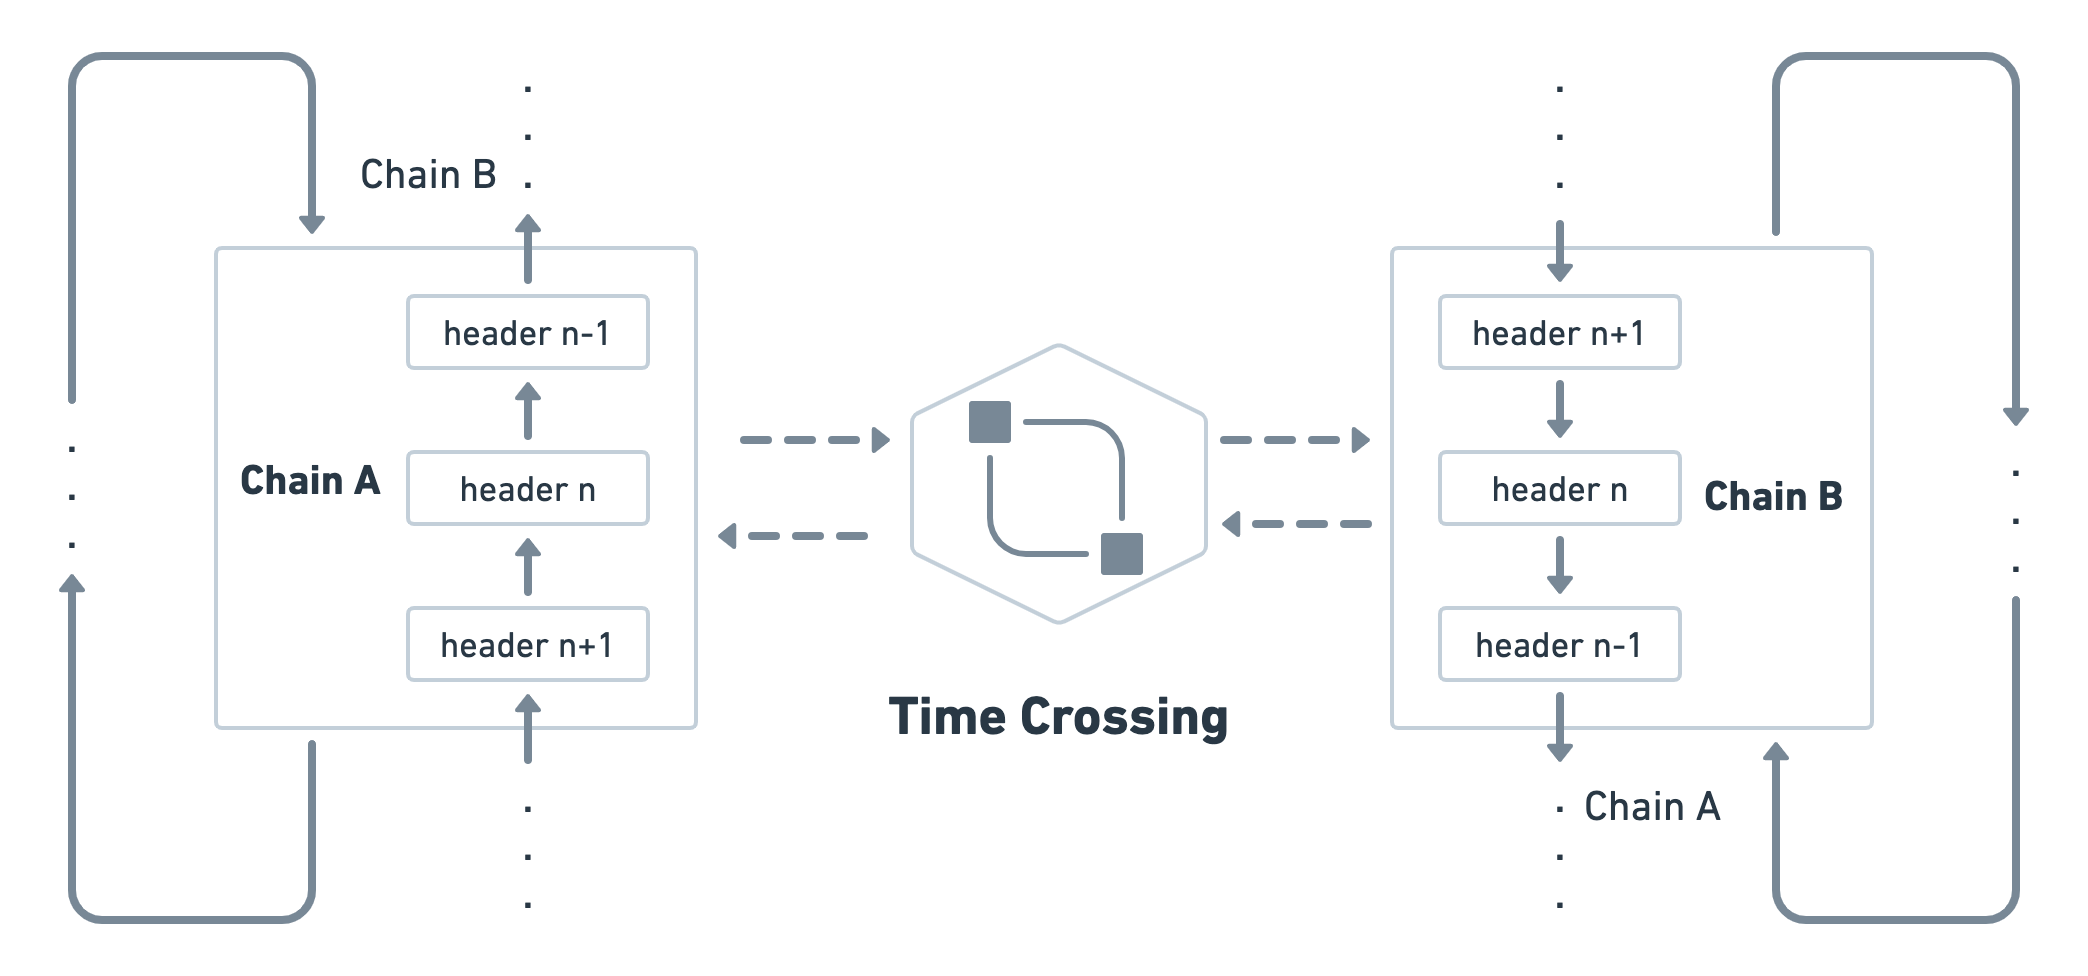
\includegraphics[width=\textwidth]{images/9.png}
	\caption{Cross-chain validation}
	\label{fig:9} 
\end{figure}

\subsection{Multi-chain Structure}
With the cross-chain protocol, \texttt{Cube} has the ability to support multiple chain structures. Applications can build their own application chains using the settlement layer as a template, allowing for greater customization, which is ideal for GameFi-related projects. In addition, being multi-chain helps in scalability, as \texttt{Cube} has theoretically almost unlimited scalability through continuous relaying and bridging.

\subsection{Cross Channel: Cross-chain Contract Calls}
In addition to cross-chain assets, \texttt{Cube} also supports cross-chain contract calls, meaning that DeFi applications from one chain can be directly called from another chain. \texttt{Cube} has defined a Cross Channel protocol to handle contract calls between chains.


\subsubsection{Shadow Account}
Shadow Account is a key part of Cross Channel. As the name implies, it is a shadow account of the source chain account in the target chain, which represents the source chain account operating in the target chain.
The Shadow Account is generated in a deterministic way to ensure that the source chain account corresponds to the Shadow Account, as follows.
$$address_{shadow} = address_{generate}(sha256(prefix + address_{source}))$$

The Shadow Account can be seen as a normal account of the target chain to participate in transactions.
However, Shadow Account does not have a private key, and thus differs again from a normal account in terms of transaction validation. Shadow Account transactions are generated from the cross-chain transactions. We can embed the cross-chain transaction hash when generating Shadow Account transactions, and write the generated Shadow Account transaction hash in the execution result of cross-chain transactions. After that, we can confirm the validity of the Shadow Account transaction by verifying the cross-chain transaction.

\subsubsection{Cross Channel Call Flow}
When the Shadow Account corresponding to the source chain account is created, the \texttt{Cube} can start the subsequent cross-chain call operations. First, when the cross-chain contract call transaction is packaged, the assets associated with the contract call are transferred to the Shadow Account corresponding to the source chain account, and then the Cross Channel protocol creates a new equivalent transaction with the Shadow Account as the initiator of the contract call. Then the new transaction interacts with the target chain's DeFi applications as if it were a normal transaction on the target chain. Finally, the result of the interaction is returned back from the Shadow Account to the source chain account, as follows in figure \ref{fig:10}.

\begin{figure}[h]
	\centering
	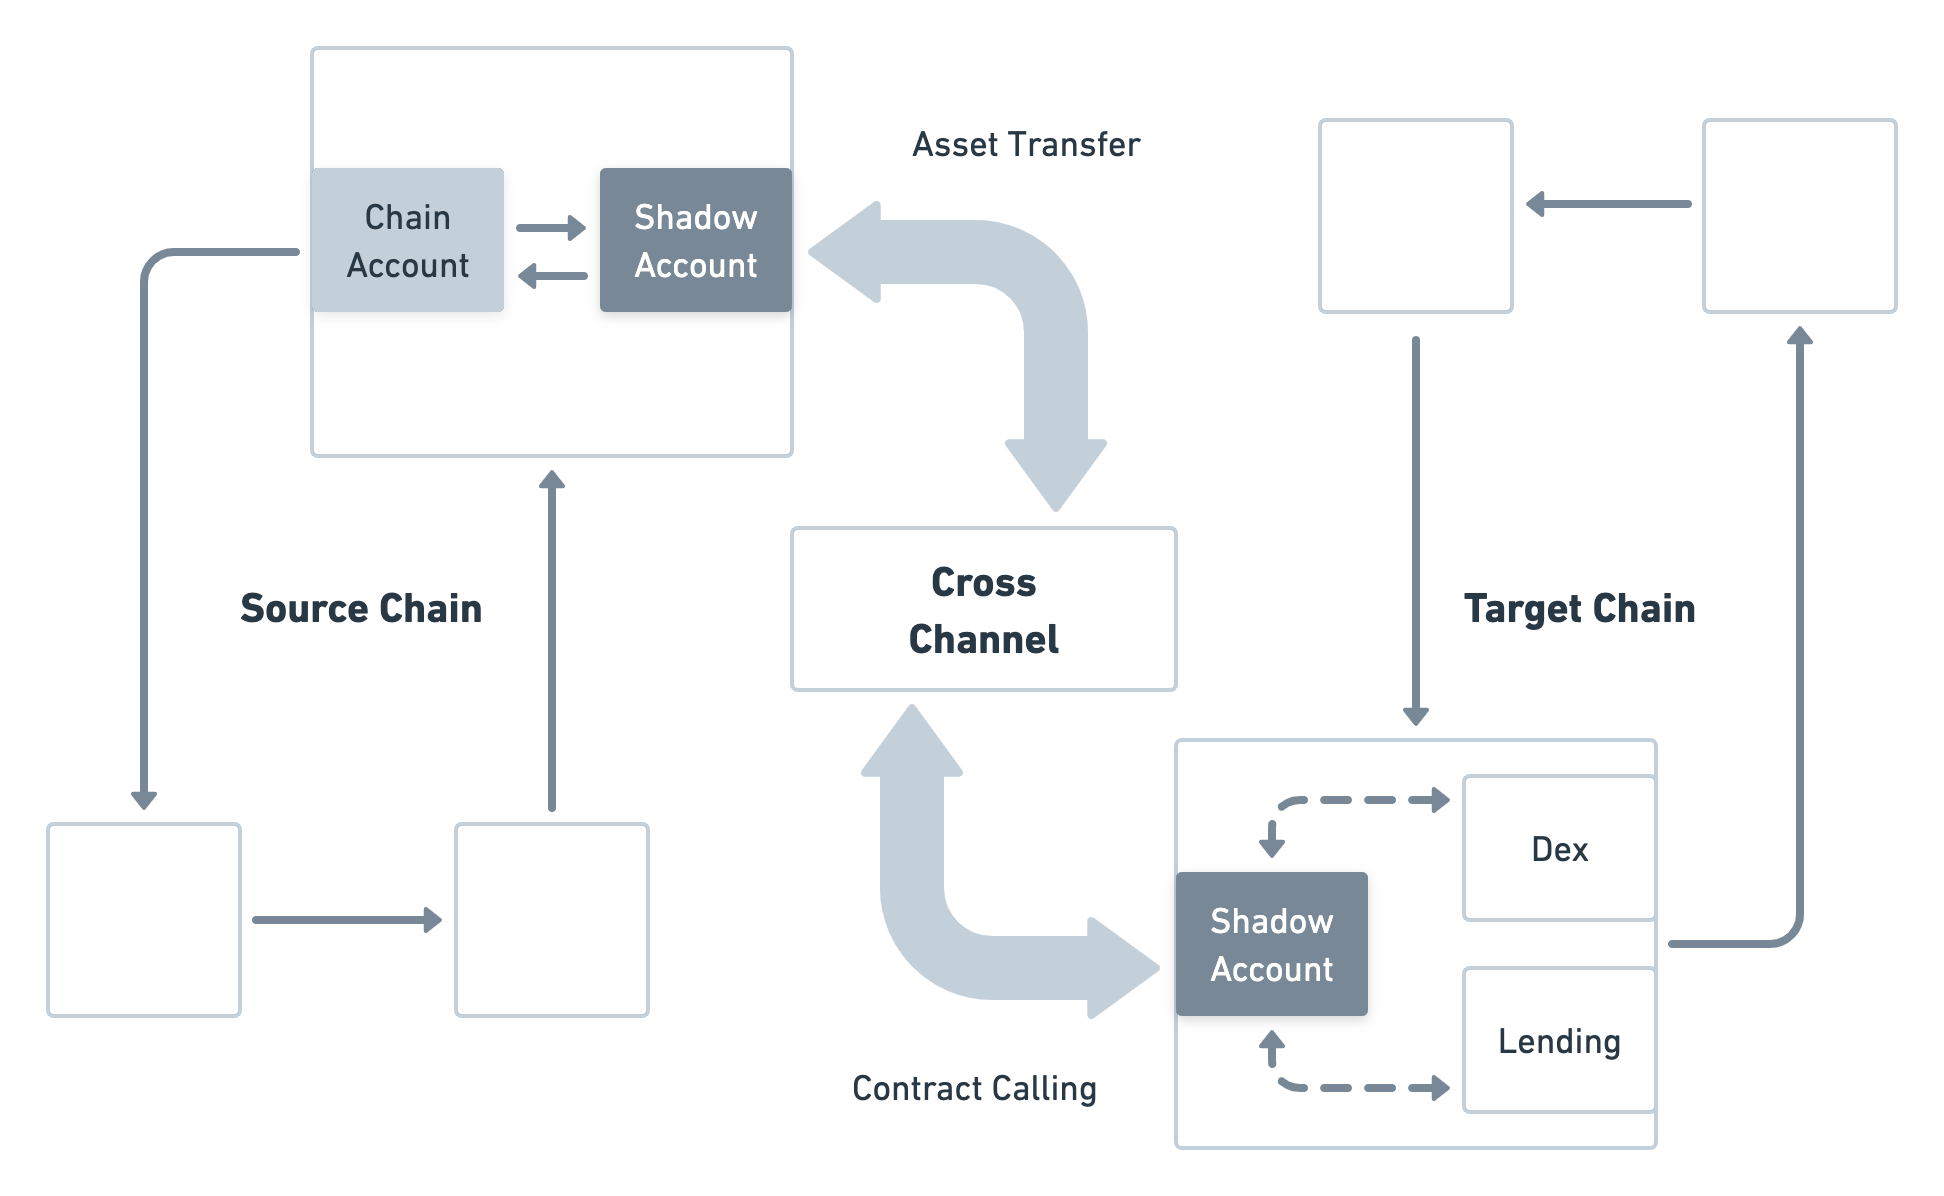
\includegraphics[width=\textwidth]{images/10.png}
	\caption{Cross-chain contract calls}
	\label{fig:10} 
\end{figure}

The idea of the Cross Channel protocol is to automate the previously required multi-step, the manual cross-chain contract calls in a verifiable way, solving the problem of cross-chain DeFi composability. 


\subsection{IBC Compatibility}
Since both Time Crossing and Cosmos IBC are based on the BFT consensus verification in terms of cross-chain validation, this makes compatibility possible. Time Crossing is fully compatible with the message format of the Cosmos IBC protocol at the cross-chain protocol level, allowing two chains to call each other. In this way, \texttt{Cube} can also access the Cosmos Hub and seamlessly cross-chain with Cosmos's various application chains, thus integrating into the Cosmos ecosystem.


\section{Future Work}
\texttt{Cube}'s future work includes the following areas:
At the execution layer, \texttt{Cube} will keep up with the latest developments in zkEVM and promote the practicality, engineering and open-source of zkEVM technology through self-research and collaboration. \texttt{Cube} will use it as the default execution engine for its chain. 
In the settlement layer, we will advance our research of consensus protocols, including semi-synchronous networks and pure asynchronous networks, to support the consensus of larger-scale consensus nodes in various network environments. 
In the data availability layer, we will continue to reduce trust assumptions and improve storage efficiency.


\section*{References}
\begin{enumerate}
	\item M. Al-Bassam, A. Sonnino, and V. Buterin, Fraud proofs: Maximising light client security and
	scaling blockchains with dishonest majorities, CoRR, vol. abs/1809.09044, 2018.
	\item E. Syta, P. Jovanovic, E. Kokoris-Kogias, N. Gailly, L. Gasser, I. Khoffi, M. J. Fischer, and B. Ford. Scalable Bias-Resistant Distributed Randomness. In the 38th IEEE Symposium on Security and Privacy, May 2017.
	\item The Ethereum Team. A note on data availability and erasure coding. https:// github.com/ethereum/research/wiki/A-note-on-data-availability-and-erasure-coding
	\item Satoshi Nakamoto. Bitcoin: A peer-to-peer electronic cash system, 2008. Available at
	https://bitcoin.org/ bitcoin.pdf
	\item The Ethereum Foundation. Ethereum Whitepaper. Available at https://github.com/ ethereum/wiki/wiki/White-Paper.
	\item E. Kokoris-Kogias, P. Jovanovic, L. Gasser, N. Gailly, E. Syta, and B. Ford, “Omniledger: A secure, scale-out, decentralized ledger via sharding,” in 2018 IEEE Symposium on Security and Privacy (SP), pp. 19–34, 2018.
	\item A. Kiayias, I. Konstantinou, A. Russell, B. David, and R. Oliynykov. Ouroboros: A provably secure proof-of-stake blockchain protocol. Cryptology ePrint Archive, Report 2016/889, 2016. http://eprint.iacr.org/.
	\item George Danezis and Sarah Meiklejohn. Centrally banked cryptocurrencies. In 23rd Annual Network and Distributed System Security Symposium, NDSS, 2016.
	\item P. Daian, R. Pass and E. Shi, Snow White: Robustly reconfigurable consensus and applications to provably secure proofs of stake, Cryptology ePrint Archive, Report 2016/919, 2017.
	\item M. Zamani, M. Movahedi, and M. Raykova, “RapidChain: A Fast Blockchain Protocol via Full Sharding.” Cryptology ePrint Archive, Report 2018/460, 2018. https://eprint.iacr.org/2018/460.
	\item Vasin, P. (2014) Blackcoin's Proof-of-Stake Protocol v2, https://blackcoin.co/ blackcoin-pos-protocolv2-whitepaper.pdf
	\item Loi Luu, Viswesh Narayanan, Chaodong Zheng, Kunal Baweja, Seth Gilbert, and Prateek Saxena. A secure sharding protocol for open blockchains. In Proceedings of the 2016 ACM SIGSAC Conference on Computer and Communications Security, CCS '16, pages 17–30, New York, NY, USA, 2016. ACM.
	\item Rafael Pass and Elaine Shi. Thunderella: Blockchains with optimistic instant confirmation. https://eprint.iacr.org/2017/913.pdf.
	\item Joseph Poon,Vitalik Buterin. Plasma: Scalable Autonomous Smart Contracts. http://plasma.io/plasma-deprecated.pdf
	\item Vitalik Buterin, “An Incomplete Guide to Rollups”, https://vitalik.ca/general /2021/01/05/rollup.html
	\item S. Dziembowski, S. Faust, and K. Hostakova, “Foundations of state channel networks.” Cryptology ePrint Archive, Report 2018/320, 2018. https:// eprint.iacr.org/2018/320.
\end{enumerate}

\end{document}
